\documentclass[conference]{IEEEtran}
\IEEEoverridecommandlockouts

\usepackage{cite}
\usepackage{amsmath,amssymb}
\usepackage{graphicx}
\usepackage{booktabs}
\usepackage{multirow}
\usepackage{xcolor}
\usepackage[hidelinks]{hyperref}

\newcommand{\A}[1]{\textsf{#1}}                         % arm identifiers
\newcommand{\pmsd}[1]{{\scriptsize$\pm$#1}}

\begin{document}

\title{Pretraining on Unlabeled Headlines Beats GAN-BERT and Helper Tasks for Sarcasm Detection with Few Labels}

% Double-blind submission: no author names, affiliations or links.
\author{\IEEEauthorblockN{Anonymous Authors}
\IEEEauthorblockA{\textit{Affiliation withheld for review}}}

\maketitle

\begin{abstract}
Labeled sarcasm data are expensive, so many detectors also learn from unlabeled text. A recent model for the News Headlines dataset combines GAN-BERT, a generator-and-discriminator method, with sentiment and emotion helper tasks and reports 93.88\% accuracy, but it does not show which part of the recipe does the work. Teams that copy it may build parts that give nothing. We take the recipe apart and test each part against plain BERT, with the same test set and label budgets from 1\% to 100\%. Used as the recipe uses them, neither the GAN nor the helper tasks beat BERT at any budget. A simpler step wins: continuing BERT's masked-word pretraining on the unlabeled training headlines. With 1\% of the labels it adds 7.4 points of macro-F1, the effect of about ten times more labels, and with three cheap add-ons it beats the recipe by 10.7 points. The advantage fades as labels grow, and on tweets labeled by their authors it is small and unreliable, so it is a finding about News Headlines. With 70\% of the labels no tested method reaches 93.88\% on a held-out test set.
\end{abstract}

\begin{IEEEkeywords}
sarcasm detection, semi-supervised learning, continued pretraining, label efficiency, GAN-BERT, controlled comparison
\end{IEEEkeywords}

% ======================================================================
\section{Introduction}

Sarcasm says the opposite of what it means, so systems that read surface sentiment get it wrong, and every labeled example costs human effort. A common answer is to learn from unlabeled text too. For the News Headlines dataset~\cite{misra2023sarcasm}, a recent model does this with GAN-BERT~\cite{croce2020ganbert}, which learns from unlabeled text through a generator--discriminator game, and with sentiment and emotion helper tasks whose labels come from pretrained classifiers. It reports 93.88\% accuracy, 1.84 points above its BERT baseline~\cite{irfan2025seed}.

The problem is that such a result credits the whole recipe and no part of it. The original report compares the recipe with BERT, LSTM and CNN models, but not with the recipe minus the GAN or minus the helper tasks. A group that wants to use unlabeled text can therefore not tell what to build. Building a generator, a pair of teacher models and a multi-task loss is slow, and if only one piece matters, the rest is wasted work. A simpler alternative is also on the table: continue BERT's own pretraining on the unlabeled text of the task before fine-tuning~\cite{gururangan2020dont}. It has been compared with self-training on topic and sentiment tasks~\cite{shi2023rethinking}, but not with the recipe above and not for sarcasm.

We take the recipe apart and put every piece, plus the simple alternative, into one controlled test. Only the method under test changes: the encoder, the step budget, the test set and the statistics stay fixed. Throughout, quality is macro-F1, the average of the F1 scores of the sarcastic and the serious class. We ask: (Q1) does the GAN or any helper task carry the recipe's gain, and what does? (Q2) How large is that gain, how stable, and how many labels does it save? (Q3) Does it hold at the label budget of the original report, and on sarcasm labeled by people other than the headline's outlet?

Our findings are:
(i) used as the recipe uses them (on labeled and unlabeled headlines), neither the GAN nor the helper tasks beat plain BERT at any tested budget, even when the GAN is given 35 times more training steps; helper heads on the labeled headlines alone help by 1.6 points at 1\% labels;
(ii) continued pretraining on the unlabeled training headlines adds 7.4 macro-F1 points at 1\% labels, matches BERT with ten times the labels, and with three cheap add-ons beats the recipe by 10.7 points at 1\% and 1.6 at 30\%;
(iii) the claim has limits: at 70\% labels all methods tie within one point, the reported 93.88\% cannot be reproduced on a held-out test set, and the gain does not appear reliably on author-labeled tweets.

% ======================================================================
\section{Related Work}

\textbf{Using unlabeled text.} GAN-BERT~\cite{croce2020ganbert} adds a generator of fake sentence vectors and a $(k{+}1)$-way discriminator~\cite{salimans2016improved}. Self-training labels unlabeled text with the model's own confident predictions~\cite{lee2013pseudo}. Semi-supervised methods can look better than they are when baselines are weak~\cite{oliver2018realistic}. Continued pretraining on the task's own text~\cite{gururangan2020dont} was found to be more robust than five self-training methods on topic and sentiment tasks~\cite{shi2023rethinking}, and on natural language understanding benchmarks it combines well with self-training~\cite{li2021tapt}. Those studies covered topic, sentiment, inference and similar tasks, not sarcasm, and not a corpus drawn from two outlets. We test whether the result holds for sarcasm, against the parts of a published sarcasm recipe.

\textbf{Affect and sarcasm.} Sentiment and emotion have served as helper tasks for sarcasm~\cite{chauhan2020sentiment}, as intermediate tasks for BERT~\cite{savini2022intermediate} and as soft targets~\cite{chen2022jointly}; the recipe we examine takes their labels from pretrained classifiers~\cite{barbieri2020tweeteval,demszky2020goemotions}. Adversarial training on word embeddings (FGM)~\cite{miyato2017adversarial} was reported to outperform semi-supervised GAN-BERT for Bengali sarcasm~\cite{zihan2026fgm}.

\textbf{Shortcuts and transfer.} In News Headlines the label equals the outlet (\textit{The Onion} or \textit{HuffPost}), a known source of shortcut learning~\cite{gururangan2018annotation,geirhos2020shortcut}, and sarcasm detectors transfer poorly across datasets~\cite{jang2024generalizable}.

% ======================================================================
\section{Experimental Design}

\subsection{Data and label budgets}
\textbf{News Headlines}~\cite{misra2023sarcasm}: after removing punctuation~\cite{irfan2025seed} and 118 duplicates, 28,501 headlines remain (47.5\% sarcastic), split into 22,800 training, 2,850 development and 2,851 test headlines. For each seed we draw nested labeled subsets $L$ of 1, 5, 10, 30, 70 and 100\% of the training set (228 to 22,800 headlines); the rest is the unlabeled pool $U$, whose labels are hidden. \textbf{iSarcasmEval}~\cite{abufarha2022semeval} (English Task~A, 1,400 test tweets labeled by their authors, 14\% sarcastic) is used for transfer and for an in-domain check.

\subsection{The recipe, taken apart}
Every run fine-tunes bert-base-uncased~\cite{devlin2019bert} with a linear sarcasm head. The original code was not available, so we re-implemented the recipe from its description; the original draws three generator--discriminator pairs and drops the neutral sentiment class, ours uses one generator on the sarcasm head and three sentiment classes (a limit of this study). Arm codes are in parentheses.
\begin{itemize}
\item \textbf{BERT} on $L$ only (\A{A1}), the baseline.
\item \textbf{GAN} (\A{A4}): GAN-BERT reading $U$. \textbf{Helper heads} on $L$ only (\A{A2}) and on $L$ and $U$ (\A{A3}), loss weight 0.3. \textbf{Full recipe} (\A{A5}): GAN plus helper heads on $L$ and $U$.
\item \textbf{Other ways to use $U$}: adversarial training with FGM (\A{A7}, $L$ only); self-training (\A{A6}: the \A{A1} model labels $U$, confident headlines are kept, a fresh model trains on $L$ plus these); a diffusion model over [CLS] vectors as the GAN's generator (\A{A24}) or as a consistency perturbation (\A{A25}); 22,417 LLM-written sarcastic/serious headline pairs as extra labeled rows (\A{A10}); and \A{A30}, helper heads + FGM + self-training together.
\item \textbf{Continued pretraining} on the 22,800 training headlines, no labels, before fine-tuning: masked-word prediction (MLM, \A{A20}; 15\% of tokens, 10,000 steps, batch 64, about 35 minutes on one T4 GPU) or a JEPA-style prediction of hidden-span representations~\cite{assran2023ijepa} (\A{A22}). Development and test headlines are never used. \A{A36} adds the three cheap add-ons of \A{A30} to the MLM encoder.
\end{itemize}
Settings tuned on development data at 10\% labels (learning rate $5{\times}10^{-5}$, helper weight, FGM size $\epsilon{=}0.5$) were frozen before any test score was computed; nothing else was tuned.

\subsection{Training and statistics}
All runs use AdamW, batch size 32, maximum length 48 and the same step budget, $\max(200, 10 \text{ passes over } L)$, with no early stopping, and training is deterministic: a re-run of 16 earlier runs reproduced their predictions exactly. Single-stage routes with a $U$ batch per step, such as the GAN, read only 28\% of one pass over $U$ at 1\% labels (200 steps $\times$ 32 of 22,572 headlines), while MLM reads about 28 passes. We therefore also test the GAN with 35 times more steps and MLM with fewer. Seeds 0--4 change the labeled subset, initialization and batch order. We report test macro-F1 (mean $\pm$ s.d.\ over seeds) and compare two methods with a paired bootstrap over test headlines~\cite{berg2012empirical} (10,000 resamples, difference of seed-averaged scores, 95\% interval); a second bootstrap that also resamples seeds is used for the main contrasts. Holm's correction~\cite{holm1979simple} is applied inside each table of contrasts; for the earliest comparisons it was computed after the fact over all 38 contrasts, and the uncorrected test was the planned one. Directional hypotheses were written before each round of experiments. Runs used one T4 GPU each (PyTorch 2.11, Transformers 5.20, Python 3.13); every run stores its code commit and library versions, and run-level predictions are released with the code.

% ======================================================================
\section{Results}
Q1 is answered by Tables~\ref{tab:main} and~\ref{tab:ours}, Q2 by Fig.~\ref{fig:curve}, and Q3 by Tables~\ref{tab:seven} and~\ref{tab:isarc}.

\begin{table}[t]
\centering
\caption{Q1: test macro-F1 (\%, mean $\pm$ s.d.\ over 5 seeds). $U$: reads the unlabeled pool. Bold: best per budget. The published recipe, re-implemented, is \A{A5}.}
\label{tab:main}
\footnotesize
\setlength{\tabcolsep}{4pt}
\begin{tabular}{llcc}
\toprule
Arm & Method & 1\% (228) & 10\% (2,280) \\
\midrule
\A{A1} & BERT & 80.4\pmsd{1.2} & 88.2\pmsd{0.3} \\
\midrule
\A{A4} & GAN-BERT ($U$) & 80.5\pmsd{1.6} & 88.1\pmsd{0.4} \\
\A{A3} & Helper heads on $L$ and $U$ & 80.3\pmsd{1.8} & 88.6\pmsd{0.5} \\
\A{A5} & GAN-BERT + helper heads ($U$) & 78.1\pmsd{2.7} & 88.4\pmsd{0.3} \\
\A{A24} & Diffusion fakes ($U$) & 80.3\pmsd{2.8} & 88.0\pmsd{0.6} \\
\A{A25} & Diffusion consistency ($U$) & 75.6\pmsd{4.8} & 87.4\pmsd{0.5} \\
\A{A10} & LLM-written pairs & 63.9\pmsd{0.8} & 73.4\pmsd{0.7} \\
\midrule
\A{A2} & Helper heads on $L$ only (H) & 82.1\pmsd{0.6} & 88.4\pmsd{0.4} \\
\A{A7} & FGM (F) & 82.0\pmsd{0.6} & 89.8\pmsd{0.1} \\
\A{A6} & Self-training (S, $U$) & 82.0\pmsd{0.7} & 88.8\pmsd{0.3} \\
\A{A30} & H + F + S ($U$) & 84.6\pmsd{0.9} & 89.9\pmsd{0.4} \\
\midrule
\A{A22} & JEPA pretraining ($U$) & 86.1\pmsd{0.3} & 89.8\pmsd{0.2} \\
\A{A20} & MLM pretraining ($U$) & 87.8\pmsd{0.5} & 91.0\pmsd{0.3} \\
\A{A36} & MLM + H + F + S ($U$) & \textbf{88.8}\pmsd{0.3} & \textbf{91.6}\pmsd{0.3} \\
\bottomrule
\end{tabular}
\end{table}

\subsection{Q1: The GAN and the recipe's helper tasks carry no gain}

\textbf{The GAN does nothing.} GAN-BERT is level with BERT at 1, 5 and 10\% ($+0.10$, $-0.11$, $-0.13$ points, all $p > 0.5$) and slightly worse at 30\% ($-0.55$, $p_{\mathrm{Holm}} = 0.053$). Giving it 35 times more steps (about 10 passes over $U$) makes it worse, not better: at 1\% it scores 7.9 points below BERT trained for the same number of steps (73.5 against 81.4, with a large seed spread), and 7.1 below itself at the normal length. The short training is therefore not the reason for its null result. Diffusion samples in place of the GAN's fakes change nothing ($-0.15$ at 1\%).

\textbf{The helper tasks do nothing in the design of the original report.} With helper heads on $L$ and $U$, as in the recipe, the change is $-0.13$ at 1\%. Only the variant on $L$ alone gains ($+1.63$ at 1\%, $p < 10^{-4}$); the difference between the two variants is $1.76$ points. The full recipe (\A{A5}) is 2.3 points \emph{below} BERT at 1\% ($p < 10^{-4}$) and level at 5, 10, 30 and 70\% ($+0.00$, $+0.23$, $-0.08$, $-0.25$). The helper labels carry almost no sarcasm signal: a probe on the teacher's eight sentiment and emotion probabilities predicts sarcasm with an AUC of 0.546. When the helper labels are shuffled across headlines, the heads still add $+1.17$ points at 1\%, 72\% of the gain with real labels. The heads act as a regularizer when labels are very scarce, not as a source of affective knowledge. On sarcastic headlines with positive surface sentiment (107 in the test set), the helper heads help slightly \emph{less} than on the others (a difference in error change of $+2.6$ [0.0, 5.1] points at 1\% and $+2.8$ [0.6, 5.1] at 10\%; after correction $p_{\mathrm{Holm}} = 0.14$ and $0.06$). This is the direction expected if the sentiment target pulls the wrong way, but it is not a significant result.

\textbf{Three cheap add-ons give about 1.6 points each at 1\%}: helper heads on $L$ ($+1.63$), FGM ($+1.58$) and self-training ($+1.62$), all $p < 10^{-4}$; at 10\% only FGM keeps its gain ($+1.55$). Together they give $+4.17$ at 1\%. LLM-written pairs cost 16.5 and 14.8 points: the generated sarcastic headlines are longer and use stock phrasing, which a model can learn instead of sarcasm.

\textbf{Continued pretraining is far stronger.} MLM adds $+7.42$ points at 1\% [6.55, 8.32] and $+2.80$ at 10\% [2.09, 3.53], every seed ahead, and beats the three add-ons together by 3.2 points at 1\%. When seeds are resampled as well, the 1\% gain stays between $+6.18$ and $+8.68$. JEPA helps ($+5.67$, $+1.63$) but trails MLM on every seed.

\begin{table}[t]
\centering
\caption{Q1: our best recipe (\A{A36}) against the recipe from the original report (\A{A5}, re-implemented). Test macro-F1 (\%), mean over 5 seeds; difference with 95\% paired-bootstrap interval, all $p_{\mathrm{Holm}}<0.05$.}
\label{tab:ours}
\footnotesize
\setlength{\tabcolsep}{5pt}
\begin{tabular}{lccc}
\toprule
Labels & \A{A36} & \A{A5} & \A{A36} $-$ \A{A5} \\
\midrule
1\%  & 88.81 & 78.12 & $+10.68$ [9.58, 11.84] \\
5\%  & 90.61 & 86.62 & $+3.99$ [3.14, 4.82] \\
10\% & 91.60 & 88.44 & $+3.15$ [2.37, 3.93] \\
30\% & 92.41 & 90.77 & $+1.64$ [1.01, 2.26] \\
\bottomrule
\end{tabular}
\end{table}

Table~\ref{tab:ours} puts our best recipe against the original one: the gap is 10.7 points at 1\% and still 1.6 at 30\%. With seeds resampled, the 1\% interval is [8.57, 13.36]. About 7.4 of the 8.4 points that \A{A36} gains over BERT at 1\% come from pretraining. On the pretrained encoder, the three add-ons each add nothing significant (helper heads $+0.48$, FGM $-0.09$, self-training $+0.35$), because pretraining absorbs their gains; together they add $+0.97$ [0.39, 1.54] at 1\% and nothing that survives correction at 10\%. Adding the GAN and helper heads on top of the pretrained encoder (\A{A37}) \emph{lowers} the score by $1.20$ [0.69, 1.70] at 1\%.

\subsection{Q2: How large, how stable, how many labels saved}

\begin{figure}[t]
\centering
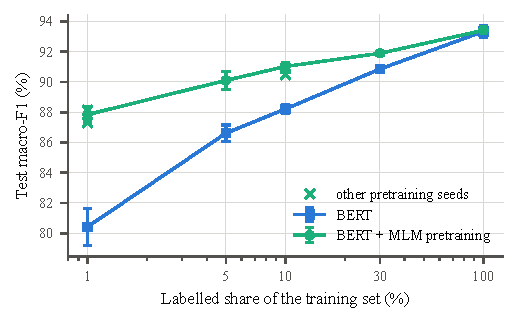
\includegraphics[width=\columnwidth]{figures/fig_curve.pdf}
\caption{Q2: test macro-F1 against the label budget (log scale), mean $\pm$ s.d.\ over 5 seeds. Crosses: MLM pretraining repeated with two other pretraining seeds.}
\label{fig:curve}
\end{figure}

\textbf{Stability.} We pretrained twice more with other seeds. The three encoders give $+7.42$, $+7.72$ and $+6.89$ points over BERT at 1\% and $+2.80$, $+2.68$ and $+2.26$ at 10\%, all with every fine-tuning seed ahead (Fig.~\ref{fig:curve}).

\textbf{Label efficiency.} The gain shrinks as labels grow: $+3.49$ at 5\%, $+1.04$ at 30\% and $+0.09$ with every label (not significant). With 1\% of the labels the pretrained model is level with BERT trained on 10\% ($-0.38$ [$-1.15$, 0.41]), so it saves roughly a factor of eight to ten in labels there. Reading BERT's own curve (straight lines between budgets on a log scale), BERT would need 4.4, 3.3 and 1.7 times more labels to match the pretrained model at 5, 10 and 30\%. These are ``no significant difference'' results, not proofs of equality.

\textbf{More pretraining, more gain.} At 1\% labels the gain over BERT is $-0.36$ after 100 steps (the GAN's exposure to $U$, 6,400 headlines), $+1.66$ after 350, $+3.08$ after 1,000, $+5.24$ after 3,000 and $+7.42$ after 10,000 steps. Exposure matters for MLM, but it does not rescue the GAN, which gets worse with more steps (Q1).

\subsection{Q3: Where the claim stops}

\begin{table}[t]
\centering
\caption{Q3: the original report's regime, 70\% of the training labels. Test accuracy and macro-F1 (\%), mean over 5 seeds; $p_{\mathrm{H}}$: Holm-adjusted.}
\label{tab:seven}
\footnotesize
\setlength{\tabcolsep}{5pt}
\begin{tabular}{lccc}
\toprule
Arm & Acc. & F1 & F1 vs.\ \A{A1} \\
\midrule
\A{A1} BERT & 92.76 & 92.74 & \\
\A{A5} Full recipe & 92.51 & 92.49 & $-0.25$ (n.s.) \\
\A{A20} MLM pretraining & 93.16 & 93.15 & $+0.41$ (n.s.) \\
\A{A7} FGM & 93.40 & 93.38 & $+0.64$ ($p_{\mathrm{H}}{=}0.02$) \\
\bottomrule
\end{tabular}
\end{table}

\textbf{The reported 93.88\% is not reproduced.} At 70\% of the labels (the original report's regime) the four methods lie within 0.9 points (Table~\ref{tab:seven}), and the recipe is below the other three. No tested method reaches 93.88\% on our held-out test set; the best is FGM at 93.40, and FGM reaches 93.90 only with all labels. The reported figure also cannot be placed on our scale. The original Table~II lists a support of 28,619 for every model, the size of the whole dataset, so its numbers appear to be computed over training headlines as well. We scored BERT and the recipe on all rows, training headlines included, and accuracy rises by 3.9 to 4.0 points at 70\% labels (96.5 for the recipe) and by 5.3 at full labels (98.6) because the model has memorized its training rows. Those numbers are 2.6 to 4.7 points above 93.88, so the protocol alone does not explain it either; we only conclude that 93.88\% is not a held-out accuracy.

\textbf{Outlet words.} In News Headlines the label is the outlet. We masked the 200 words most indicative of the outlet (100 per class, chosen on the training set) and, as a control, the same number of random words. Every BERT model loses about 3 points more under cue masking; pretrained models show the same gap (difference from BERT $-0.07$ at 1\%, $-0.17$ at 10\%, none significant). Pretraining makes the model better at this dataset; it does not make it rely less on outlet vocabulary.

\begin{table}[t]
\centering
\caption{iSarcasmEval test ROC-AUC (\%), mean over 10 seeds, with $N$ labeled tweets. MLM on the tweets' own unlabeled text (\A{A20}) against BERT (\A{A1}).}
\label{tab:isarc}
\footnotesize
\setlength{\tabcolsep}{5pt}
\begin{tabular}{lccc}
\toprule
$N$ & \A{A1} & \A{A20} & difference [95\% CI] \\
\midrule
228   & 52.6 & 51.3 & $-1.33$ [$-3.71$, 1.07] \\
780   & 55.5 & 57.9 & $+2.45$ [0.06, 4.87] \\
3,120 & 66.0 & 67.9 & $+1.95$ [$-0.23$, 4.18] \\
\bottomrule
\end{tabular}
\end{table}

\textbf{Author-labeled tweets.} Headlines carry the outlet as label, so we repeated the test on iSarcasmEval, whose tweets are labeled by their authors: MLM on the unlabeled training tweets, BERT and MLM fine-tuned on $N$ = 228, 780 and 3,120 labeled tweets (Table~\ref{tab:isarc}; AUC is the area under the ROC curve, 50 is chance). The gain is not reliable. It is negative at 228 labels, where BERT is near chance (AUC 52.6) and a gain could not be seen anyway, and $+2.45$ at 780, whose interval just excludes zero but does not survive correction ($p_{\mathrm{Holm}} = 0.45$). The Headlines encoder is level with the in-domain one at 228 and 780 labels (differences $+0.08$ and $+0.20$). More pretraining (100 instead of 28.7 passes) changes nothing ($+0.38$, $-0.10$). A control with an encoder pretrained on a random 3,120-headline subset, the size of the tweet pool, keeps $+3.00$ of the full pool's $+7.4$ at 1\% labels: a small pool explains a large part of the smaller gain, though not all. Models pretrained on headlines also stay near chance on iSarcasmEval without any tweet labels (AUC 47.8 to 57.3), below a rule that scores each tweet by its word count alone (68.7).

% ======================================================================
\section{Discussion}

\textbf{What to use when labels are scarce.} Before building generators or helper tasks, continue pretraining the encoder on the unlabeled text already at hand. In our tests this took about 35 minutes of one GPU, needed no extra model or data, and gave the largest gain at every budget up to 30\%. The recipe's GAN and helper tasks, as used there, add nothing over BERT in our re-implementation; pretraining is the piece that matters. This agrees with results on topic and sentiment tasks~\cite{gururangan2020dont,shi2023rethinking,li2021tapt}; what we add is that it holds for sarcasm, against the parts of a published sarcasm recipe.

\textbf{What the gain means.} The gain is label efficiency on News Headlines. The pretrained model learns the dataset faster, outlet vocabulary included, and it does not transfer. A two-outlet corpus is the ideal case for continued pretraining, because outlet style is exactly what masked-word prediction learns from the unlabeled text. The weak result on iSarcasmEval fits that reading, though it also fits a small pool and a noisy, hard test set, and we cannot separate the two. High scores on this dataset should not be read as sarcasm understanding.

\textbf{Limitations and threats to validity.} (i) One encoder size, one main dataset and one author-labeled check with low ceiling; JEPA used one pretraining seed. (ii) Our recipe is a re-implementation from the paper's description, with one generator instead of three and three sentiment classes instead of two. Our statements concern that re-implementation. They say nothing about the original code, and the original numbers are not comparable with ours (different split, different scoring). (iii) The GAN with long training was tried with one schedule and one learning rate; its instability was not diagnosed. (iv) The bootstrap resamples test headlines (and, for the main contrasts, seeds); cross-budget comparisons pair different labeled subsets. (v) The sentiment audit used a single annotator.

% ======================================================================
\section{Conclusion}

In our re-implementation of a published sarcasm recipe, the GAN and the helper tasks, used as the recipe uses them, give nothing over plain BERT at any tested budget. Continuing BERT's masked-word pretraining on the unlabeled training headlines gives far more: 7.4 macro-F1 points with 1\% of the labels, and 10.7 points over the recipe once three cheap add-ons are included. The gap closes as labels grow and does not carry reliably to author-labeled tweets. For practitioners with few labels and plenty of unlabeled text: pretrain on that text first, and test any extra component against that baseline. Future work should ablate each part of a combined recipe and score on held-out data.

\bibliographystyle{IEEEtran}
\bibliography{refs}

\end{document}
